\newcommand{\kdtreebboxfig}{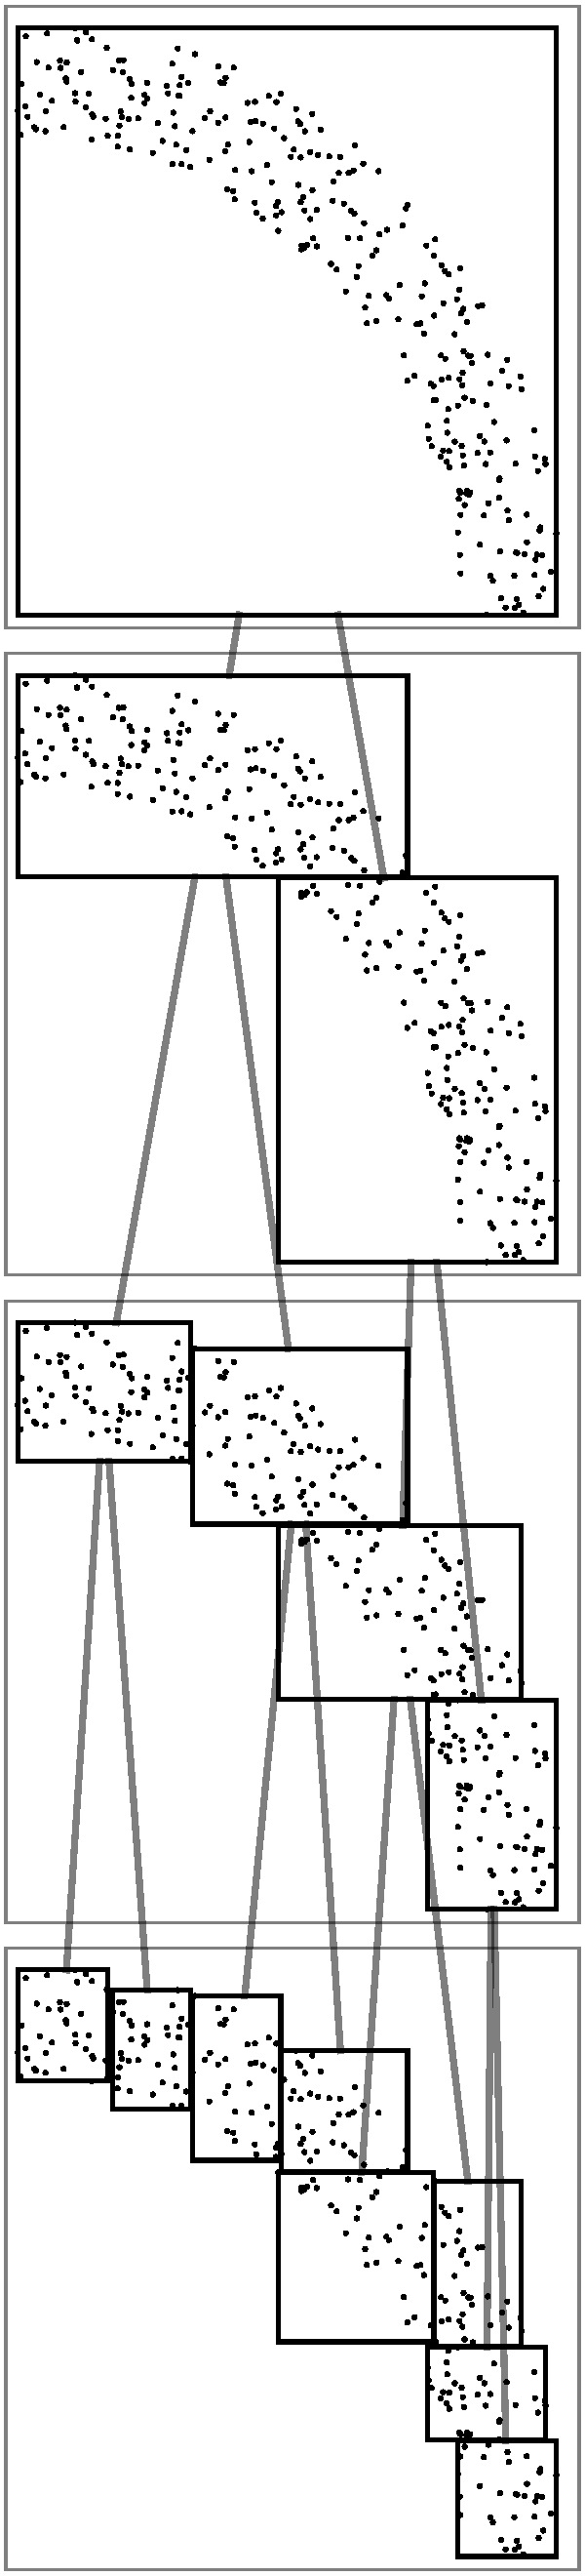
\includegraphics[width=1.000000\figunit]{kdtree-bbox}}
\newcommand{\kdtreesplitfig}{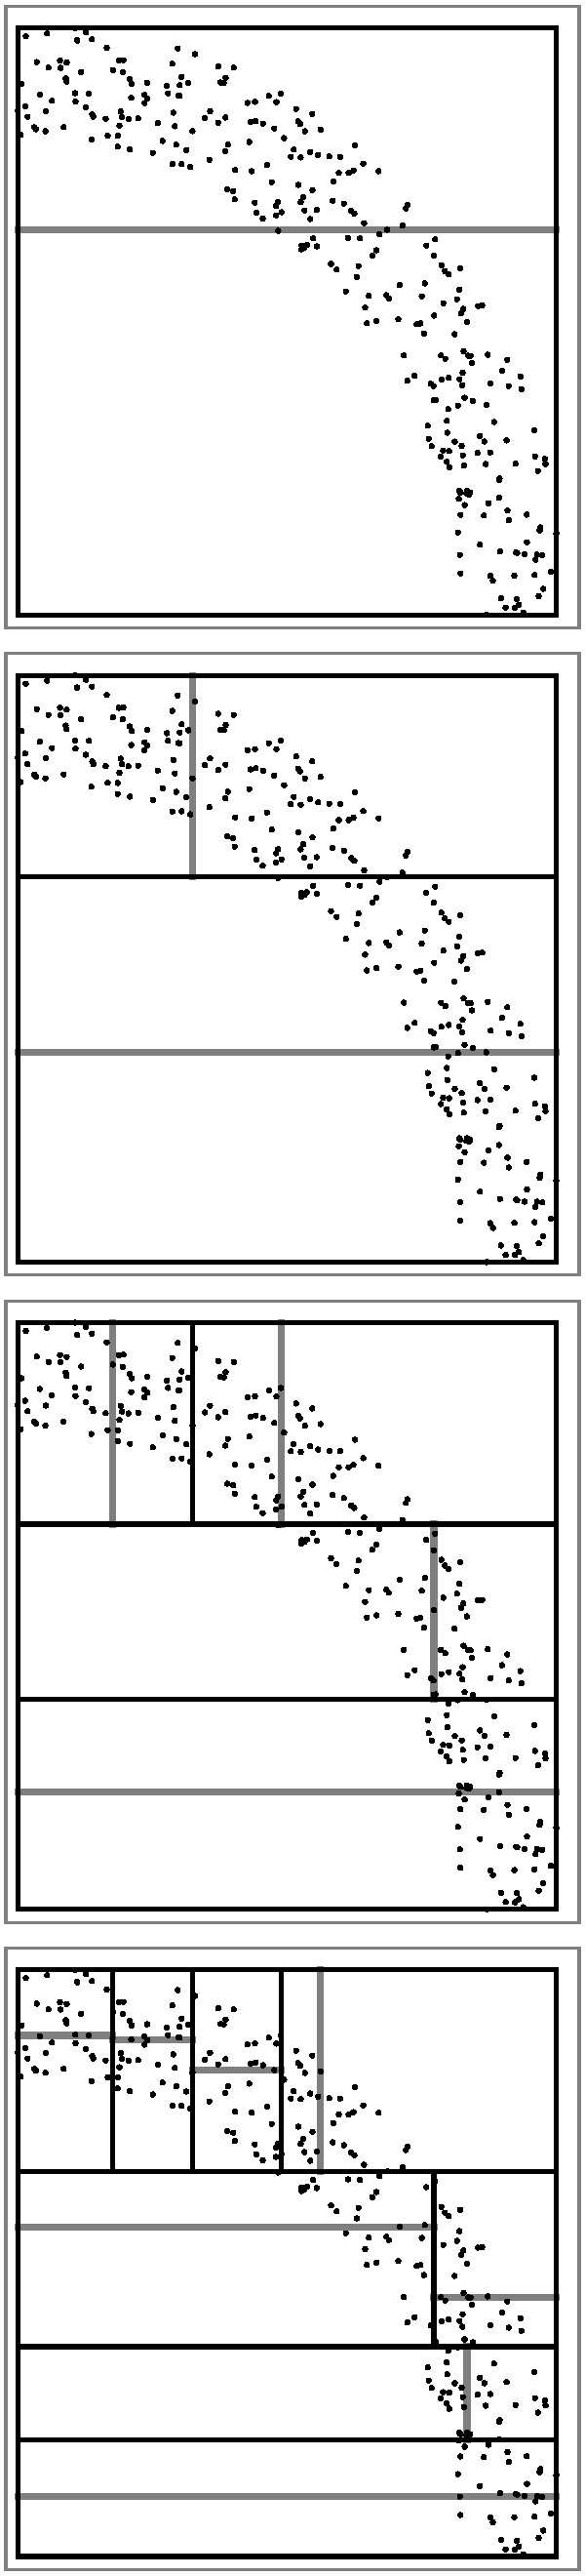
\includegraphics[width=1.000000\figunit]{kdtree-split}}
\newcommand{\mindistbboxfig}{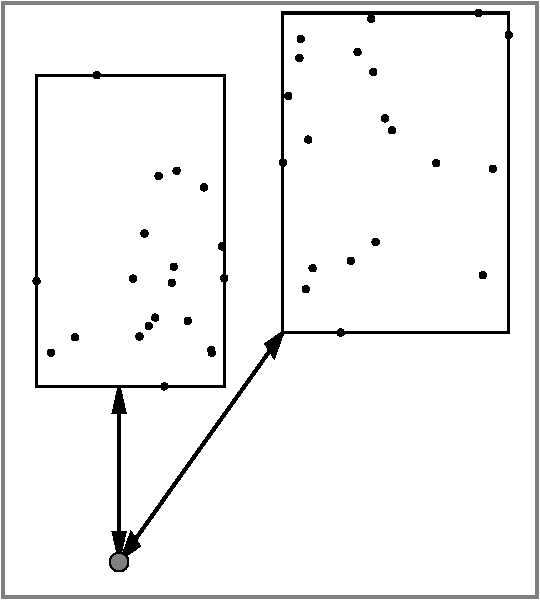
\includegraphics[width=0.900000\figunit]{mindist-bbox}}
\newcommand{\mindistsplitfig}{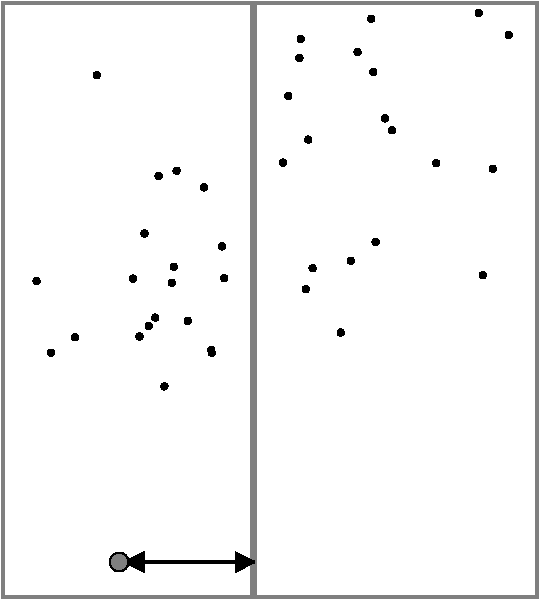
\includegraphics[width=0.900000\figunit]{mindist-split}}
%% see   getbb.sh  to find the bounding-box of the ink in a figure.

%% The sizes shown are from getbb.sh using 12pt font in figures.

%% pgf/tikz often believes that the bounding-box extends beyond the
%% extent of the ink, so forcing it to the ink size doesn't always
%% work (the figure overflows onto page 2)

% 169 x 65
\newcommand{\pointerlessfigwidth}{170pt}
\newcommand{\pointerlessfigheight}{76pt}

% 267 x 249
\newcommand{\permutefigwidth}{268pt}
\newcommand{\permutefigheight}{249pt}

% 251 x 162
\newcommand{\applypermfigwidth}{252pt}
\newcommand{\applypermfigheight}{162pt}

% 263 x 119
\newcommand{\ronlyfigwidth}{268pt}
\newcommand{\ronlyfigheight}{122pt}

% 233 x 93
\newcommand{\transposefigwidth}{234pt}
\newcommand{\transposefigheight}{93pt}

% 145 x 58
\newcommand{\bitpackfigwidth}{149pt}
\newcommand{\bitpackfigheight}{66pt}

\newcommand{\kdbarmemfig}{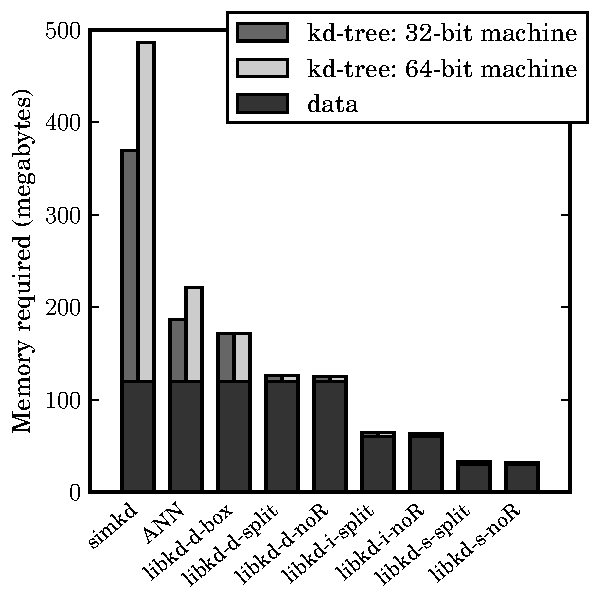
\includegraphics[width=1.000000\figunit]{kd-bar-mem}}
\newcommand{\kdbarspeedfig}{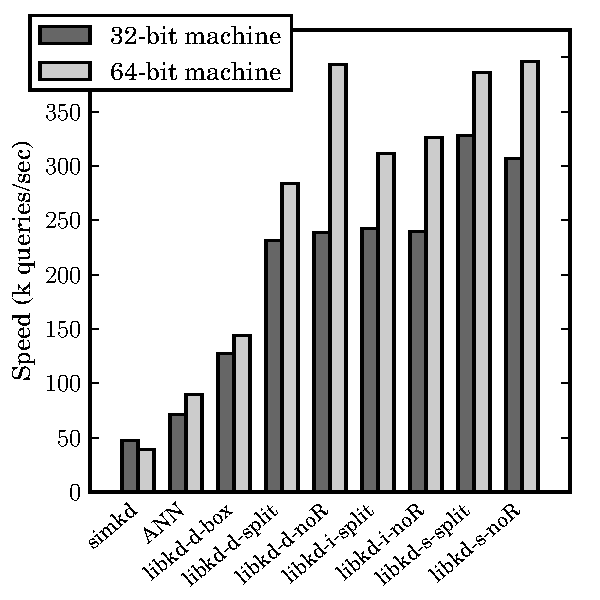
\includegraphics[width=1.000000\figunit]{kd-bar-speed}}
